\chapter{Plastisitas Saraf, Pembelajaran, dan Ingatan}\label{ch:b3:learning-memory}

Pada tahun 1953 seorang ahli bedah membuang bagian dalam kedua lobus temporal
seorang pemuda yang epilepsinya tak tertangani. Kejangnya mereda; pasiennya,
yang selama lima puluh tahun dikenal sebagai H.M., tidak pernah membentuk lagi
sebuah ingatan yang bertahan tentang sebuah kejadian. Ia dapat bercakap-cakap,
belajar menjiplak sebuah bintang di dalam sebuah cermin sebaik siapa pun --- lalu
tiap hari menyangkal pernah melihat tugas itu --- dan ia mengingat masa kecilnya.
Ingatan, ternyata, bukanlah satu hal, dan pembuatan ingatan baru tentang kejadian
bergantung pada sebuah struktur sebesar ibu jari. Apa yang berubah di dalam sebuah
otak ketika ia belajar adalah pertanyaan tertua ilmu saraf, dan jawabannya, yang
digarap pada seekor siput laut berneuron dua puluh ribu dan pada irisan \omterm{def:b3:learning-memory:kinds}{hipokampus}
tikus, adalah bahwa sinapsis mengubah kekuatannya menurut apa
yang lewat melaluinya --- sebuah kaidah yang ditebak Donald Hebb pada tahun 1949 dan
sebuah molekul, yakni \omterm{prop:b3:learning-memory:nmda}{reseptor NMDA}, yang ternyata melaksanakannya. Bab ini
memperlakukan kaidah itu dan mesinnya, sirkuit yang memakainya untuk menyimpan
tempat dan kejadian, matematika yang mengatakan apa yang dapat dipelajari sistem
semacam itu dan berapa banyak yang dapat dimuatnya, serta isyarat ganjaran yang
memberitahunya apa yang layak dipelajari.

\section{Jenis ingatan dan tempat tinggalnya}

\begin{definition}[Bentuk pembelajaran dan ingatan]\label{def:b3:learning-memory:kinds}
\index{pembiasaan}\index{pemekaan}\index{pelaziman}\index{ingatan deklaratif}%
\index{ingatan prosedural}\index{pemantapan}\index{hipokampus}
Pembelajaran yang paling sederhana bersifat \emph{takasosiatif}: \emph{pembiasaan},
yakni sebuah tanggapan yang menurun terhadap sebuah rangsang tak berbahaya yang berulang, dan
\emph{pemekaan}, yakni sebuah tanggapan yang menguat sesudah sebuah rangsang yang merugikan.
Pembelajaran \emph{asosiatif} menghubungkan dua kejadian: pada \emph{pelaziman
klasik} (Pavlov) sebuah rangsang netral yang meramalkan sebuah ganjaran atau
hukuman berakhir memicu tanggapannya; pada \emph{pelaziman operan}
sebuah tindakan yang diganjar diulang. Ingatan manusia
terbagi menjadi ingatan \emph{deklaratif} --- fakta dan kejadian, yang teringat
secara sadar, yang bergantung pada \emph{hipokampus} dan lobus temporal
medial --- dan ingatan \emph{nondeklaratif} --- keterampilan dan kebiasaan
(striatum, \omterm{def:b3:nervous-systems:plan}{otak kecil}), rasa takut yang terlazimkan (amigdala), pemrimaan (korteks)
--- yang diungkapkan dalam kinerja tanpa pengingatan. Sebuah ingatan dipegang
mula-mula dalam sebuah bentuk jangka pendek yang labil, yang bertahan beberapa detik sampai jam, lalu
\emph{dimantapkan} sepanjang jam sampai tahun menjadi sebuah bentuk jangka panjang yang mantap
yang tidak lagi memerlukan hipokampusnya dan tinggal di dalam korteksnya.
\end{definition}

\begin{proof}[Bukti eksperimental]
Scoville dan Milner (1957) melaporkan H.M.: sesudah pembuangan kedua
\omterm{def:b3:learning-memory:kinds}{hipokampusnya} dan korteks di sebelahnya, kecerdasannya dan
ingatannya dari sebelum pembedahannya sebagian besar utuh, ingatan kerjanya
normal selama ia memperhatikan sesuatu, tetapi ia tidak dapat
membentuk ingatan baru tentang kejadian atau fakta apa pun. Ia mempelajari keterampilan motorik pada
laju yang normal sepanjang hari sambil menyangkal pernah berlatih --- sehingga
ingatan keterampilannya tidak memerlukan \omterm{def:b3:learning-memory:kinds}{hipokampus} --- dan ia mengingat masa
lampau yang jauh lebih baik daripada tahun-tahun tepat sebelum pembedahannya, sehingga \omterm{def:b3:learning-memory:kinds}{hipokampusnya}
diperlukan untuk meletakkan dan untuk sementara waktu memegang \omterm{def:b3:learning-memory:kinds}{ingatan deklaratif}, bukan untuk
menyimpannya selamanya. Monyet dan tikus dengan lesi yang serupa menunjukkan
pemisahan yang sama, dan kajian seorang pasien tunggal menata ulang
bidangnya.
\end{proof}

\section{Kaidah Hebb dan molekulnya}

\begin{definition}[Plastisitas Hebb, LTP, dan LTD]\label{def:b3:learning-memory:ltp}
\index{kaidah Hebb}\index{potensiasi jangka panjang}%
\index{depresi jangka panjang}\index{plastisitas bergantung-saat-lecutan}
Hebb (1949) mengusulkan bahwa ketika sebuah neuron prasinapsis berulang kali ikut
serta menyalakan neuron pascasinapsis, sambungan di antara keduanya
diperkuat --- ``sel yang menyala bersama terangkai bersama''.
\emph{Potensiasi jangka panjang} (LTP) adalah bentuk percobaannya: sebuah
ledakan singkat rangsangan berfrekuensi tinggi pada sebuah jalur membuat sinapsis
yang diaktifkannya lebih kuat selama berjam-jam pada sebuah irisan dan berminggu-minggu pada seekor
hewan. LTP bersifat \emph{khas-masukan} (hanya sinapsis yang dirangsang yang
berubah), \emph{asosiatif} (sebuah masukan lemah yang dipasangkan dengan sebuah masukan kuat ke
sel yang sama dipotensiasi), dan memerlukan \emph{\omterm{def:b3:structural-biology:allostery}{kekooperatifan}} di antara
masukannya untuk mendepolarisasi selnya. \emph{Depresi jangka panjang} (LTD) adalah
lawannya, yang dihasilkan keaktifan berfrekuensi rendah yang berkepanjangan. Pada
\emph{plastisitas bergantung-saat-lecutan} tandanya ditetapkan urutannya: sebuah
lecutan prasinapsis beberapa milidetik \emph{sebelum} lecutan pascasinapsisnya
memperkuat sinapsisnya, satu yang tepat \emph{sesudahnya} melemahkannya, di dalam
sebuah jendela sekitar \qty{20}{ms} pada tiap sisinya --- sehingga sebuah sinapsis
belajar meramalkan, bukan sekadar berkorelasi.
\end{definition}

\begin{proposition}[Reseptor NMDA sebagai pendeteksi kebetulan]\label{prop:b3:learning-memory:nmda}
\index{reseptor NMDA}\index{reseptor AMPA}%
\index{CaMKII}\index{CREB}\index{duri dendrit}
Pada sinapsis pemacu, glutamat bekerja pada dua reseptor. Reseptor
\emph{AMPA} terbuka begitu mengikat lalu mengusung arus
sinapsis yang biasa. Reseptor \emph{NMDA} mengikat glutamat tetapi
terhalang pada potensial istirahat oleh sebuah ion magnesium di dalam liangnya; hanya ketika
selaput pascasinapsisnya terdepolarisasi --- oleh banyak masukan sekaligus, atau
oleh sebuah potensial aksi yang merambat balik --- magnesiumnya terusir
dan salurannya menghantar, lalu memasukkan kalsium. \omterm{prop:b3:learning-memory:nmda}{Reseptor NMDA} dengan demikian
terbuka hanya ketika pelepasan prasinapsis (glutamat) berbarengan dengan
keaktifan pascasinapsis (depolarisasi): ia gerbang ``dan'' milik Hebb di dalam
sebuah protein tunggal. Kalsium yang memasuki sebuah \emph{\omterm{prop:b3:learning-memory:nmda}{duri dendrit}}
mengaktifkan kinase \emph{CaMKII}, yang memfosforilasi \omterm{prop:b3:learning-memory:nmda}{reseptor AMPA}
lalu mendorong lebih banyak dari reseptor itu ke dalam sinapsisnya dari sebuah cadangan --- sinapsisnya
lebih kuat dalam hitungan menit (LTP awal). Sebuah kenaikan kalsium yang besar dan lambat
justru mengaktifkan fosfatase kalsineurin, yang menyingkirkan \omterm{prop:b3:learning-memory:nmda}{reseptor
AMPA}: itulah LTD. Potensiasi yang bertahan lebih daripada beberapa jam (LTP akhir)
memerlukan protein baru: kinasenya mencapai intinya, faktor transkripsi
\emph{CREB} menyalakan gen, lalu durinya tumbuh dan dapat terbelah ---
yakni tuntutan yang sama akan pengungkapan gen yang memisahkan ingatan jangka pendek
dari jangka panjang pada tiap hewan yang dikaji.
\end{proposition}

\begin{proof}[Bukti eksperimental]
Bliss dan L\o mo (1973) merangsang jalur perforan ke dalam
\omterm{def:b3:learning-memory:kinds}{hipokampus} kelinci dengan sebuah deretan denyut lalu menemukan tanggapan
yang terbangkitkan membesar selama berjam-jam sesudahnya --- yakni LTP yang pertama. Collingridge
(1983) menunjukkan bahwa sebuah penghalang \omterm{prop:b3:learning-memory:nmda}{reseptor NMDA} (AP5) mencegah
pengimbasan LTP tetapi bukan tanggapan sinapsis yang biasa; Morris (1986)
memasukkan AP5 ke dalam \omterm{def:b3:learning-memory:kinds}{hipokampus} tikus lalu menemukan bahwa mereka tidak lagi
dapat mempelajari kedudukan sebuah panggung tersembunyi di dalam sebuah kolam air sambil
berenang dan melihat secara normal; dan mencit yang \omterm{prop:b3:learning-memory:nmda}{reseptor NMDA-nya}
dihapus hanya di daerah \omterm{def:b3:learning-memory:hippocampus}{CA1} \omterm{def:b3:learning-memory:kinds}{hipokampusnya} tidak punya LTP di sana
maupun ingatan ruang. Reseptor yang sama, di tempat yang sama, diperlukan
bagi perubahan sinapsisnya dan bagi pembelajarannya.
\end{proof}

\begin{omfigure}
\begin{tikzpicture}[every node/.style={font=\scriptsize}, >=stealth]
  % presynaptic terminal
  \draw[thick, omDef, fill=omDef!12] (0,2.2) .. controls (0,3.4) and (4,3.4) .. (4,2.2) -- (4,1.7) -- (0,1.7) -- cycle;
  \node at (2,2.8) {terminal prasinapsis};
  \foreach \p in {(0.8,2.0),(1.6,2.1),(2.6,2.0),(3.3,2.1)} \draw[thick, fill=omDef!40] \p circle (0.17);
  \foreach \p in {(1.2,1.45),(2.0,1.5),(2.9,1.42)} \fill[omProp] \p circle (0.06);
  \node[right, omProp] at (3.3,1.45) {glutamat};
  % postsynaptic spine
  \draw[thick, omMeth!70!black, fill=omMeth!10] (-0.6,1.1) -- (4.4,1.1) -- (4.4,-1.2) -- (-0.6,-1.2) -- cycle;
  \node at (0.6,-0.9) {duri dendrit};
  % AMPA
  \draw[thick, fill=omMeth!45] (0.2,0.85) rectangle (0.6,1.35); \node[below, align=center] at (0.1,0.8) {AMPA:\\Na$^{+}$ masuk};
  \draw[->, thick] (0.4,1.7) -- (0.4,0.95);
  % NMDA with Mg
  \draw[thick, fill=omThm!35] (2.4,0.85) rectangle (2.9,1.35); \fill[gray!70] (2.65,1.1) circle (0.09); \node[right, font=\tiny] at (2.95,1.1) {halangan Mg$^{2+}$};
  \node[below, align=center] at (2.65,0.8) {NMDA: memerlukan glutamat\\\emph{dan} depolarisasi};
  \draw[->, thick, omThm] (2.65,0.15) -- (2.65,-0.5) node[below] {Ca$^{2+}$};
  % downstream
  \node[draw, rounded corners, fill=omThm!15, font=\tiny] (cam) at (5.6,0.3) {CaMKII};
  \draw[->, thick] (2.9,-0.5) -- (cam);
  \node[draw, rounded corners, fill=omMeth!25, font=\tiny, align=center] (ampa) at (8.2,1.0) {lebih banyak reseptor AMPA\\disisipkan: LTP awal (menit)};
  \node[draw, rounded corners, fill=omMeth!25, font=\tiny, align=center] (creb) at (8.2,-0.5) {CREB, protein baru,\\duri tumbuh: LTP akhir (jam+)};
  \draw[->, thick] (cam) -- (ampa.west); \draw[->, thick] (cam) -- (creb.west);
  \node[draw, rounded corners, fill=omDef!15, font=\tiny, align=center] (ltd) at (8.2,-1.8) {Ca$^{2+}$ lambat dan kecil: kalsineurin,\\AMPA disingkirkan: LTD};
  \draw[->, thick, dashed] (2.9,-0.7) .. controls (4.5,-1.6) .. (ltd.west);
\end{tikzpicture}

{\small \omterm{prop:b3:learning-memory:nmda}{Reseptor NMDA} sebagai gerbang Hebb. Glutamat sendiri membuka \omterm{prop:b3:learning-memory:nmda}{reseptor
AMPA}; saluran NMDA menghantar hanya ketika durinya juga
terdepolarisasi dan magnesiumnya pergi. Kalsium yang lalu masuk menetapkan
masa depan sinapsisnya: sebuah kenaikan yang cepat dan besar memperkuatnya, sebuah kenaikan yang lambat dan kecil
melemahkannya.}
\end{omfigure}

\begin{omfigure}
\begin{tikzpicture}
\begin{axis}[
  width=6.6cm, height=5.2cm,
  axis x line=bottom, axis y line=left,
  xmin=-20, xmax=120, ymin=0, ymax=220,
  xlabel={menit}, ylabel={tanggapan sinapsis (\%)},
  xlabel style={font=\small, at={(axis description cs:0.5,-0.12)}, anchor=north}, ylabel style={font=\small},
  tick label style={font=\scriptsize}, xtick={0,30,60,90,120}, ytick={0,100,200},
  clip=false,
]
\addplot[only marks, mark=*, mark size=1pt, omDef] coordinates {(-18,100) (-15,98) (-12,102) (-9,99) (-6,101) (-3,100) (2,195) (5,180) (8,172) (11,168) (15,165) (20,162) (30,160) (40,158) (50,157) (60,156) (70,156) (80,155) (90,155) (100,154) (110,154) (120,154)};
\addplot[only marks, mark=o, mark size=1pt, gray] coordinates {(-18,100) (-12,101) (-6,99) (2,102) (8,100) (15,101) (30,100) (45,99) (60,101) (75,100) (90,100) (105,101) (120,100)};
\draw[->, thick, omThm] (axis cs:0,215) -- (axis cs:0,200); \node[font=\scriptsize, omThm, anchor=south] at (axis cs:0,216) {tetanus};
\node[font=\scriptsize, omDef, anchor=south west] at (axis cs:35,168) {jalur yang dirangsang: LTP};
\node[font=\scriptsize, gray, anchor=north west] at (axis cs:35,95) {jalur kendali: tak berubah};
\end{axis}
\begin{axis}[
  at={(7.6cm,0)}, anchor=south west,
  width=6.6cm, height=5.2cm,
  axis x line=middle, axis y line=middle,
  xmin=-60, xmax=60, ymin=-60, ymax=100,
  xlabel={$t_{\text{pra}} - t_{\text{pasca}}$ (ms)}, ylabel={$\Delta w$ (\%)},
  xlabel style={font=\small, at={(axis description cs:0.5,-0.06)}, anchor=north}, ylabel style={font=\small, at={(axis description cs:0.5,1.02)}, anchor=south},
  tick label style={font=\scriptsize}, xtick={-40,-20,20,40}, ytick={-40,40,80},
  clip=false,
]
\addplot[very thick, omMeth!70!black, domain=-60:-0.5, samples=60] {80*exp(x/15)};
\addplot[very thick, omThm, domain=0.5:60, samples=60] {-45*exp(-x/25)};
\node[font=\scriptsize, omMeth!70!black, anchor=south east] at (axis cs:-8,62) {pra sebelum pasca: LTP};
\node[font=\scriptsize, omThm, anchor=north west] at (axis cs:8,-22) {pasca sebelum pra: LTD};
\end{axis}
\end{tikzpicture}

{\small Kiri: \omterm{def:b3:learning-memory:ltp}{potensiasi jangka panjang} --- sesudah sebuah tetanus singkat,
tanggapan jalur yang dirangsang tetap membesar selama berjam-jam sementara sebuah
jalur yang tidak dirangsang ke sel yang sama tidak berubah (kekhasan
masukan). Kanan: jendela saat lecutannya --- sinapsisnya
menguat bila lecutan prasinapsisnya memimpin dan melemah bila ia tertinggal.}
\end{omfigure}

\begin{theorem}[Apa yang dipelajari sebuah sinapsis Hebb]\label{thm:b3:learning-memory:hebb}
\index{pembelajaran Hebb!komponen utama}\index{kaidah Oja}
Misalkanlah sebuah neuron menerima masukan $\mathbf{x} = (x_{1},\dots,x_{n})$ lewat
bobot $\mathbf{w}$ lalu menanggapi secara linear, $y = \mathbf{w}\cdot\mathbf{x}$.
\omterm{def:b3:learning-memory:ltp}{Kaidah Hebb}, $\Delta\mathbf{w} = \eta\, y\,\mathbf{x}$, memberi rata-rata
atas masukannya
\[
\langle\Delta\mathbf{w}\rangle = \eta\,C\,\mathbf{w}, \qquad C =
\langle\mathbf{x}\mathbf{x}^{\mathsf{T}}\rangle ,
\]
dengan $C$ adalah matriks korelasi masukannya. Bobotnya tumbuh
tanpa batas, dan tumbuh paling cepat sepanjang vektor eigen $C$ yang
nilai eigennya terbesar: sinapsisnya berakhir mendeteksi pola masukan
yang paling sering hadir --- yakni \emph{komponen utama}
masukannya. Dengan sebuah suku yang menghukum bobot yang besar, yakni \emph{\omterm{thm:b3:learning-memory:hebb}{kaidah Oja}}
$\Delta\mathbf{w} = \eta\, y\,(\mathbf{x} - y\,\mathbf{w})$, vektor bobotnya
memusat ke vektor eigen itu yang dinormalkan ke panjang satuan, dan
neuronnya menjadi sebuah pendeteksi yang mantap bagi korelasi yang menguasai apa yang
dilihatnya.
\end{theorem}
\begin{proof}
Dengan menyulihkan $y = \mathbf{w}\cdot\mathbf{x} = \mathbf{x}^{\mathsf{T}}
\mathbf{w}$ ke dalam \omterm{def:b3:learning-memory:ltp}{kaidah Hebb} diperoleh $\Delta\mathbf{w} = \eta\,\mathbf{x}
\mathbf{x}^{\mathsf{T}}\mathbf{w}$, yang rata-ratanya atas masukannya (dengan
$\mathbf{w}$ berubah lambat) adalah $\eta C\mathbf{w}$. $C$ simetris dan
semidefinit positif, sehingga ia punya vektor eigen ortogonal $\mathbf{e}_{k}$
bernilai eigen $\lambda_{k} \ge 0$; dengan menulis $\mathbf{w} = \sum_{k}
a_{k}\mathbf{e}_{k}$, tiap komponennya memenuhi $\Delta a_{k} = \eta\lambda_{k}
a_{k}$ lalu tumbuh sebagai $(1 + \eta\lambda_{k})^{t}$, sehingga komponen sepanjang
nilai eigen terbesarnya berakhir menguasai arah $\mathbf{w}$
sementara panjangnya membesar tanpa batas. \omterm{thm:b3:learning-memory:hebb}{Kaidah Oja} merata-rata menjadi $\eta(C\mathbf{w} -
(\mathbf{w}^{\mathsf{T}}C\mathbf{w})\mathbf{w})$; pada sebuah titik tetap
$C\mathbf{w} = (\mathbf{w}^{\mathsf{T}}C\mathbf{w})\mathbf{w}$, sehingga
$\mathbf{w}$ sebuah vektor eigen dengan $\lambda = \mathbf{w}^{\mathsf{T}}
C\mathbf{w} = \lambda|\mathbf{w}|^{2}$, sehingga $|\mathbf{w}| = 1$; titik
tetap sepanjang nilai eigen terbesarnya adalah yang mantap (sebuah
gangguan ke arah vektor eigen lain menyusut, sebab nilai eigen vektor
itu lebih kecil), yang diakui saja di sini.
\end{proof}

\begin{example}[Dua masukan]\label{ex:b3:learning-memory:two-inputs}
Sebuah neuron menerima dua masukan yang biasanya aktif bersama, sehingga $C =
\begin{pmatrix} 1 & 0.8 \\ 0.8 & 1\end{pmatrix}$. Vektor eigennya adalah
$(1,1)/\sqrt{2}$ bernilai eigen $1.8$ dan $(1,-1)/\sqrt{2}$ bernilai
eigen $0.2$. Mulai dari $\mathbf{w} = (1, 0)$, \omterm{def:b3:learning-memory:ltp}{kaidah Hebb} sesudah
banyak langkah kecil memutar $\mathbf{w}$ ke arah $(1,1)$: neuronnya belajar
menanggapi kedua masukannya \emph{bersama-sama}, lalu mengabaikan kesempatan
langka yang padanya hanya satu yang menyala --- ia telah memetik korelasinya.
Dengan \omterm{thm:b3:learning-memory:hebb}{kaidah Oja} bobotnya menetap pada $(0.71, 0.71)$. Inilah maksud
bahwa sinapsis Hebb mempelajari apa yang berjalan bersama, dan itulah sebabnya
sifat asosiatif LTP, yakni memasangkan sebuah masukan lemah dengan yang kuat,
menyusul dari kaidahnya.
\end{example}

\section{Seekor siput yang belajar}

\begin{proposition}[Pemekaan pada \emph{Aplysia}]\label{prop:b3:learning-memory:aplysia}
\index{Aplysia}\index{fasilitasi prasinapsis}\index{cAMP}\index{PKA}
Siput laut \emph{Aplysia} menarik insangnya ketika sifonnya
disentuh, yakni sebuah refleks beberapa lusin neuron yang dapat dikenali. Sebuah sengatan pada
ekornya \emph{memekakannya}: penarikan terhadap sebuah sentuhan ringan menguat,
selama beberapa menit sesudah satu sengatan dan berminggu-minggu sesudah beberapa sengatan. Kandel dan
rekannya (dasawarsa 1970-an--1990-an) menelusuri perubahannya ke sinapsis antara
neuron indra sifonnya dan neuron motorik insangnya. Sengatan ekornya
memacu sebuah \omterm{def:b3:nervous-systems:cells}{interneuron} yang melepaskan serotonin ke terminal neuron
indranya; serotoninnya menaikkan AMP siklik, yang mengaktifkan
protein kinase A, yang memfosforilasi lalu menutup sebuah saluran kalium;
potensial aksi terminalnya melebar, lebih banyak kalsium masuk, dan lebih banyak
penghantar dilepaskan tiap lecutan --- itulah \emph{\omterm{prop:b3:learning-memory:aplysia}{fasilitasi prasinapsis}},
yakni sebuah perubahan kovalen yang bertahan beberapa menit. Sengatan yang berulang mengirim kinasenya ke
intinya, tempat ia mengaktifkan CREB, yang menyalakan gen yang
membangun terminal sinapsis baru: ingatan jangka panjangnya adalah lebih banyak sinapsis,
dan ia dihalangi penghambat sintesis protein yang diberikan selama
latihannya tetapi bukan sesudahnya. \emph{\omterm{def:b3:learning-memory:kinds}{Pembiasaan}} adalah lawannya,
yakni sebuah depresi sinapsis yang sama; dan \emph{\omterm{def:b3:learning-memory:kinds}{pelaziman} klasik},
yakni memasangkan sentuhannya dengan sengatannya, memperkuat fasilitasi pada
sinapsis yang aktif tepat sebelum serotoninnya tiba --- yakni sebuah
kebetulan Hebb yang dilaksanakan secara prasinapsis, oleh sebuah adenilil
siklase yang dirangsang kalsium dan serotonin bersama-sama.
\end{proposition}

\begin{omfigure}
\begin{tikzpicture}[every node/.style={font=\scriptsize}, >=stealth]
  \node[draw, thick, rounded corners, fill=omDef!20, minimum width=2cm] (sn) at (0,0) {neuron indra sifon};
  \node[draw, thick, rounded corners, fill=omMeth!25, minimum width=2cm] (mn) at (6.2,0) {neuron motorik insang};
  \node[draw, thick, rounded corners, fill=omProp!30, align=center] (in) at (2.8,2.4) {interneuron pemfasilitasi\\(serotonin)};
  \node[left] at (-2.1,0) {sentuhan}; \draw[->, thick] (-2.0,0) -- (sn);
  \draw[->, very thick] (sn) -- (mn) node[pos=0.45, below, align=center, font=\tiny] {sinapsis\\yang berubah};
  \draw[->, thick] (mn) -- (8.4,0) node[right] {insang ditarik};
  \node[above] at (2.8,3.1) {sengatan ekor}; \draw[->, thick] (2.8,3.05) -- (in);
  \draw[->, thick, omProp] (in) -- (2.8,0.25);
  \node[right, align=left, font=\tiny] at (6.6,1.6) {serotonin $\to$ cAMP $\to$ PKA $\to$\\saluran K$^{+}$ tertutup $\to$ lecutan melebar,\\Ca$^{2+}$ naik, penghantar yang naik (menit);\\berulang: PKA $\to$ CREB $\to$\\terminal baru (minggu)};
\end{tikzpicture}

{\small Sirkuit \omterm{def:b3:learning-memory:kinds}{pemekaan} \emph{Aplysia}. Serotonin dari sebuah
\omterm{def:b3:nervous-systems:cells}{interneuron} bekerja pada terminal indranya, dan sinapsis yang sama mengusung
ingatan jangka pendeknya sebagai sebuah saluran terfosforilasi dan ingatan jangka
panjangnya sebagai terminal baru.}
\end{omfigure}

\begin{omfigure}
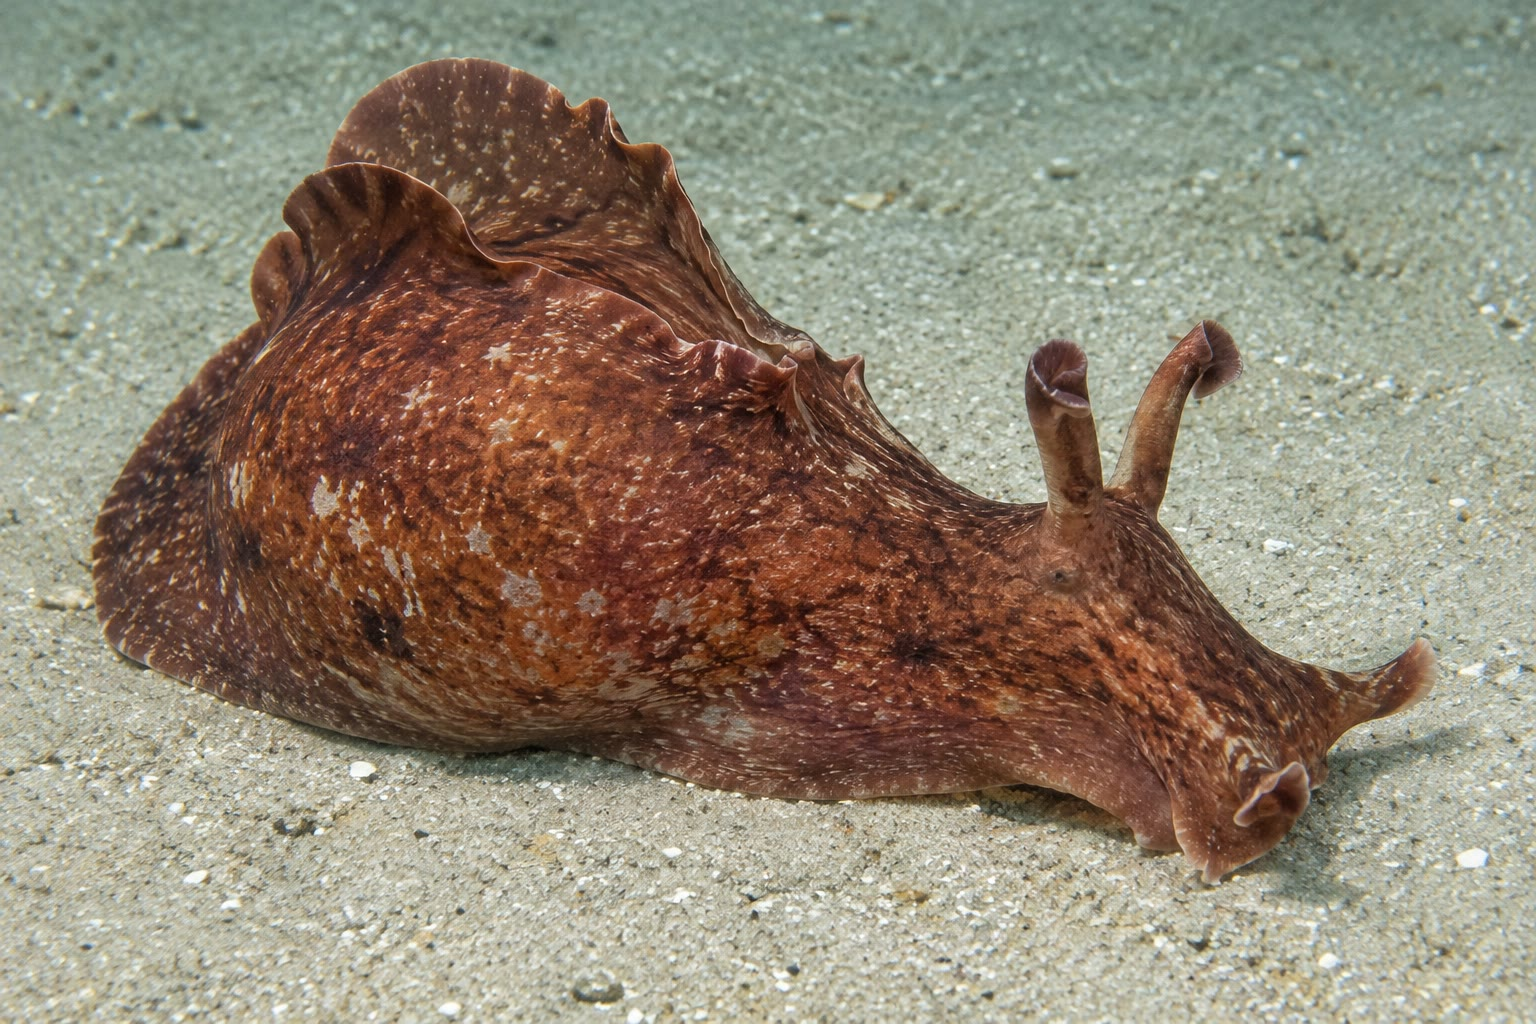
\includegraphics[width=0.46\linewidth]{images/book5/ai/b5-19-aplysia.jpg}\hspace{0.04\linewidth}
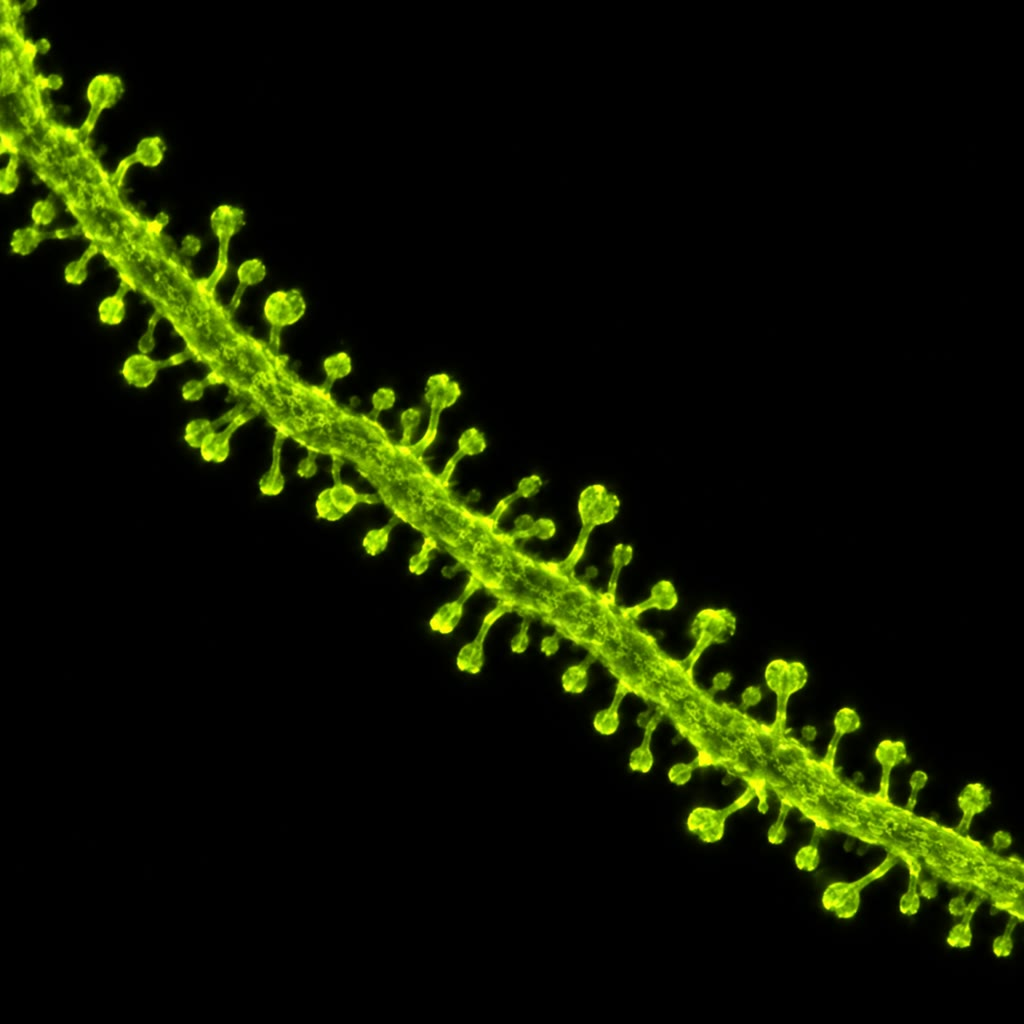
\includegraphics[width=0.36\linewidth]{images/book5/ai/b5-19-dendritic-spines.jpg}

{\small Kiri: \emph{Aplysia californica}, yang neuronnya yang sedikit dan besar
memungkinkan sinapsis sebuah ingatan ditemukan dan direkam. Kanan: sebuah dendrit
yang bertabur duri, masing-masing sisi pascasinapsis satu sinapsis pemacu
dan masing-masing sebuah petak yang kalsiumnya memutuskan nasibnya sendiri.}
\end{omfigure}

\section{Sirkuit bagi tempat dan kejadian}

\begin{definition}[Sirkuit hipokampus]\label{def:b3:learning-memory:hippocampus}
\index{girus dentatus}\index{CA3}\index{CA1}\index{sel tempat}%
\index{sel kisi}\index{pelengkapan pola}\index{pemutaran ulang}
Masukan korteks mencapai \omterm{def:b3:learning-memory:kinds}{hipokampusnya} lewat korteks entorinalnya
lalu melewati tiga tahap: \emph{girus dentatus}, yang
sel granulnya melebihi cacah masukannya lalu menyala dengan jarang (yang memisahkan
pola yang serupa); \emph{CA3}, yang sel piramidalnya saling
bersambung secara berulang, masing-masing menerima ribuan sinapsis dari
yang lain --- yakni sebuah jaringan \emph{swaasosiatif} yang dapat melengkapi sebuah
pola tersimpan dari sebuah serpihan; dan \emph{CA1}, yang membandingkan keluaran CA3
dengan masukan langsungnya lalu mengembalikan hasilnya ke korteksnya. Pada seekor tikus
yang menjelajahi sebuah arena, sebuah sel piramidal \omterm{def:b3:learning-memory:kinds}{hipokampus} menyala hanya ketika
hewannya berada di satu tempat --- yakni sebuah \emph{sel tempat} (O'Keefe, 1971) --- dan
beberapa ratus di antaranya memetakan arenanya; di dalam korteks entorinal di hulunya,
\emph{sel kisi} (Moser, 2005) menyala pada simpul sebuah kisi
segi enam yang meliputi ruangnya, yakni sebuah sistem koordinat yang darinya medan tempatnya
dibangun. Selama tidur dan istirahat, urutan sel tempat yang
menyala selama sebuah lari \emph{diputar ulang} pada laju tinggi, dan menghalangi
pemutaran ulangnya merusak ingatan larinya: \omterm{def:b3:learning-memory:kinds}{hipokampusnya} melatih ulang
jalan sehari itu kepada korteksnya.
\end{definition}

\begin{omfigure}
\begin{tikzpicture}[every node/.style={font=\scriptsize}, >=stealth]
  % trisynaptic loop
  \node[draw, thick, rounded corners, fill=gray!15, align=center] (ec) at (0,0) {korteks entorinal\\(sel kisi)};
  \node[draw, thick, rounded corners, fill=omDef!20, align=center] (dg) at (3.2,1.4) {girus dentatus:\\pemisahan pola};
  \node[draw, thick, rounded corners, fill=omProp!30, align=center] (ca3) at (7.2,1.4) {CA3, berulang:\\pelengkapan pola};
  \node[draw, thick, rounded corners, fill=omMeth!25, align=center] (ca1) at (7.2,-1.4) {CA1:\\membandingkan, mengeluarkan};
  \draw[->, thick] (ec) -- (dg); \draw[->, thick] (dg) -- (ca3); \draw[->, thick] (ca3) -- (ca1); \draw[->, thick] (ca1) -- (ec) node[pos=0.3, below, sloped, font=\tiny] {kembali ke korteks};
  \draw[->, thick, dashed] (ec) -- (ca1.north west) node[pos=0.7, above, sloped, font=\tiny] {jalur langsung};
  \draw[->, thick, omProp!80!black] (ca3.north) .. controls (6.6,2.6) and (7.8,2.6) .. (ca3.north east) node[pos=0.5, above, font=\tiny] {kolateral berulang};
  % place field map
  \begin{scope}[xshift=10.4cm, yshift=-0.2cm]
    \draw[thick] (0,0) rectangle (3,2.4); \node[below] at (1.5,-0.05) {arena, dilihat dari atas};
    \foreach \p/\c in {(0.7,1.8)/omThm, (2.1,1.9)/omDef, (1.4,0.9)/omMeth, (2.5,0.6)/omProp} { \fill[\c!60] \p circle (0.32); \fill[\c!90] \p circle (0.16); }
    \node[above] at (1.5,2.45) {medan penyalaan empat sel tempat};
  \end{scope}
\end{tikzpicture}

{\small Kiri: gelung \omterm{def:b3:learning-memory:kinds}{hipokampusnya} --- pemisahan di dalam \omterm{def:b3:learning-memory:hippocampus}{girus dentatus},
penyimpanan dan pelengkapan di dalam \omterm{def:b3:learning-memory:hippocampus}{CA3} yang berulang, perbandingan di dalam \omterm{def:b3:learning-memory:hippocampus}{CA1}. Kanan:
tiap \omterm{def:b3:learning-memory:hippocampus}{sel tempat} menyala di satu daerah sebuah arena; bersama-sama mereka memetakan
ruangnya.}
\end{omfigure}

\begin{proposition}[Berapa banyak yang dimuat sebuah jaringan swaasosiatif]\label{prop:b3:learning-memory:capacity}
\index{jaringan Hopfield}\index{kapasitas ingatan}
Sebuah jaringan berisi $N$ neuron, masing-masing tersambung ke semua yang lain dengan
bobot Hebb $w_{ij} \propto \sum_{\mu}\xi_{i}^{\mu}\xi_{j}^{\mu}$
yang dijumlahkan atas pola biner tersimpan $\xi^{\mu}$, memanggil kembali sebuah pola
tersimpan dari sebuah isyarat yang rusak atau sebagian dengan menetap ke dalamnya sebagai sebuah
penarik (Hopfield, 1982). Ia melakukannya dengan andal bagi sampai sekitar $P
\approx 0.14N$ pola acak; di luar itu polanya saling mengganggu dan
pemanggilannya runtuh. \omterm{def:b3:learning-memory:hippocampus}{CA3} seekor tikus, dengan sekitar $3\times 10^{5}$ sel
piramidal, menurut taksiran ini dapat memuat sekitar $4\times 10^{4}$ pola ---
seorde dengan tempat atau babak berbeda yang dijumpai seekor hewan dalam
semusim --- dan penyalaannya yang jarang (beberapa persen selnya aktif pada sembarang
pola) menaikkan kapasitasnya lebih jauh. \omterm{def:b3:learning-memory:hippocampus}{Pelengkapan pola} dari sebuah isyarat adalah
apa yang membuat sebuah bau atau sebuah sudut memanggil sebuah pemandangan utuh; harganya adalah bahwa
ingatan yang serupa melebur, yang ditentang pemisahan \omterm{def:b3:learning-memory:hippocampus}{girus dentatusnya}.
\end{proposition}
\admitted

\begin{method}[Menguji ingatan dan mekanismenya]\label{met:b3:learning-memory:tests}
\index{labirin air Morris}\index{pelaziman rasa takut}\index{engram}
(1) Sebuah tugas ruang: \omterm{met:b3:learning-memory:tests}{labirin air Morris} --- seekor tikus berenang di dalam air
buram menuju sebuah panggung yang tersembunyi di sebuah tempat tetap, mempelajari kedudukannya dari
isyarat ruangannya sepanjang hari, lalu diuji lewat waktu yang dihabiskan mencari
kuadran yang benar ketika panggungnya dibuang; lesi \omterm{def:b3:learning-memory:kinds}{hipokampus},
penghalang NMDA, dan hilangnya LTP masing-masing meniadakan pembelajarannya. (2) Sebuah
tugas asosiatif: \omterm{met:b3:learning-memory:tests}{pelaziman rasa takut} --- sebuah nada yang dipasangkan dengan sebuah sengatan kaki
berakhir memicu kebekuan; ingatannya bergantung pada amigdalanya, dan sebuah
versi yang khas konteksnya pada \omterm{def:b3:learning-memory:kinds}{hipokampusnya}. (3) Sebuah uji mekanisme:
halangilah calonnya (sebuah obat, sebuah \omterm{def:b3:genetic-engineering:transgenic}{penidakaktifan gen} yang terbatas pada satu daerah dan
satu waktu) lalu tunjukkanlah bahwa pembelajarannya gagal sementara persepsi dan gerakannya tidak.
(4) Engramnya: tandailah neuron yang aktif selama pembelajarannya dengan sebuah
saluran peka cahaya (\cref{ch:b3:nervous-systems}) lalu kemudian
aktifkanlah kembali dengan cahaya --- hewannya membeku di dalam sebuah konteks yang aman, seolah
mengingat; membungkamnya menghalangi pemanggilannya. Ingatan ada di dalam sel yang
dapat dikenali dan sinapsisnya, dan dapat dihidupkan dan dimatikan.
\end{method}

\begin{omfigure}
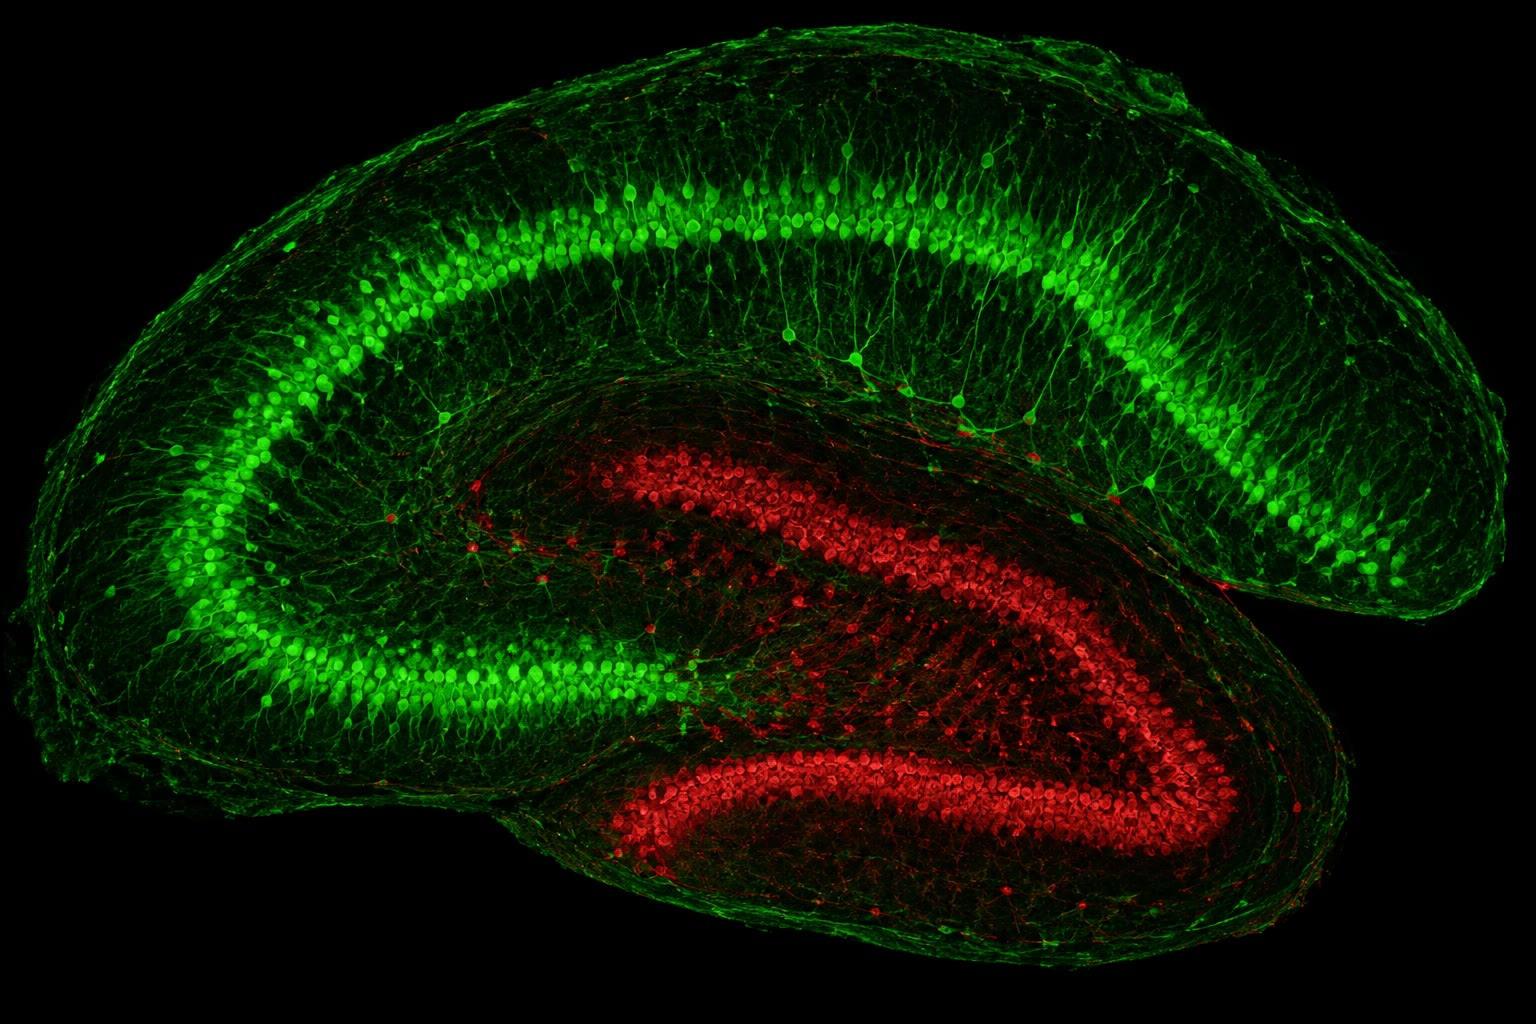
\includegraphics[width=0.56\linewidth]{images/book5/ai/b5-19-hippocampus-section.jpg}

{\small Sebuah irisan menembus \omterm{def:b3:learning-memory:kinds}{hipokampus} hewan pengerat: pita melengkung berisi
sel piramidal (hijau) dari \omterm{def:b3:learning-memory:hippocampus}{CA3} ke \omterm{def:b3:learning-memory:hippocampus}{CA1} dan \omterm{def:b3:learning-memory:hippocampus}{girus dentatus} yang saling mengunci
(merah). Tiap ingatan ruang hewannya melewati gelung
ini.}
\end{omfigure}

\section{Ganjaran, ramalan, dan plastisitas seumur hidup}

\begin{proposition}[Pembelajaran lewat galat ramalan]\label{prop:b3:learning-memory:rescorla}
\index{kaidah Rescorla--Wagner}\index{galat ramalan}\index{dopamin}
Misalkanlah $V$ nilai yang dilekatkan seekor hewan pada sebuah isyarat dan $\lambda$
ganjaran yang mengikutinya. \omterm{prop:b3:learning-memory:rescorla}{Kaidah Rescorla--Wagner} (1972) mengatakan bahwa pada
tiap percobaan nilainya berubah sebesar sebuah pecahan $\alpha$ dari
\emph{\omterm{prop:b3:learning-memory:rescorla}{galat ramalannya}}:
\[
\Delta V = \alpha\,(\lambda - V), \qquad
V_{n} = \lambda\bigl(1 - (1-\alpha)^{n}\bigr) ,
\]
sehingga pembelajarannya cepat mula-mula lalu melambat ketika ramalannya membaik,
berhenti ketika ganjarannya sepenuhnya teramalkan, lalu berbalik (pemunahan)
ketika ganjarannya ditahan. Ketika dua isyarat disajikan bersama, keduanya
berbagi satu ramalan, sehingga sebuah isyarat yang tidak menambahkan apa pun pada sebuah ramalan
yang sudah dibuat tidak dipelajari (\emph{pemblokiran}). Schultz (1997) merekam
neuron dopamin otak tengah pada monyet lalu menemukan bahwa mereka menyala
pada sebuah ganjaran tak terduga, membisu pada ganjaran yang teramalkan sepenuhnya, lalu jatuh
di bawah dasarnya ketika sebuah ganjaran yang teramalkan gagal tiba: mereka menyiarkan
$\lambda - V$, yakni \omterm{prop:b3:learning-memory:rescorla}{galat ramalannya} sendiri, ke striatum dan korteksnya,
tempat dopaminnya menggerbangkan plastisitas pada sinapsis yang belakangan ini
aktif. Mempelajari apa yang meramalkan ganjaran adalah plastisitas Hebb dengan sebuah
faktor ketiga yang mengatakan apakah hasilnya lebih baik atau lebih buruk daripada yang
diharapkan --- dan obat yang disalahgunakan, dengan menggerakkan dopamin secara langsung,
memalsukan sebuah ``lebih baik daripada yang diharapkan'' yang permanen.
\end{proposition}
\begin{proof}
Rekursi $V_{n+1} = V_{n} + \alpha(\lambda - V_{n})$ memberi
$\lambda - V_{n+1} = (1-\alpha)(\lambda - V_{n})$, sehingga galatnya menyusut
secara geometris, $\lambda - V_{n} = (1-\alpha)^{n}\lambda$ dari $V_{0} =
0$, yang darinya rumusnya berasal. Bagi dua isyarat $A$ dan $B$ yang disajikan bersama,
ramalannya adalah $V_{A} + V_{B}$; bila $A$ dilatih lebih dulu sampai
$V_{A} = \lambda$, galat pada percobaan majemuknya nol dan $B$
tidak memperoleh apa pun.
\end{proof}

\begin{omfigure}
\begin{tikzpicture}
\begin{axis}[
  width=6.6cm, height=5.0cm,
  axis x line=bottom, axis y line=left,
  xmin=0, xmax=25, ymin=0, ymax=1.1,
  xlabel={percobaan $n$}, ylabel={$V_{n}/\lambda$},
  xlabel style={font=\small, at={(axis description cs:0.5,-0.14)}, anchor=north}, ylabel style={font=\small},
  tick label style={font=\scriptsize}, xtick={0,5,10,15,20,25}, ytick={0,0.5,1},
  clip=false,
]
\addplot[very thick, omDef, domain=0:12, samples=13] {1-0.8^x};
\addplot[very thick, omDef, domain=12:25, samples=14] {(1-0.8^12)*0.8^(x-12)};
\draw[dashed, gray] (axis cs:12,0) -- (axis cs:12,1.05);
\node[font=\scriptsize, anchor=north west, align=left] at (axis cs:0.5,0.98) {ganjaran diberikan:\\perolehan};
\node[font=\scriptsize, anchor=north west, align=left] at (axis cs:14,0.98) {ganjaran ditahan:\\pemunahan};
\end{axis}
\begin{axis}[
  at={(7.6cm,0)}, anchor=south west,
  width=6.6cm, height=5.0cm,
  ybar, bar width=14pt,
  axis x line=bottom, axis y line=left,
  ymin=-1.2, ymax=1.5,
  symbolic x coords={ganjaran tak terduga, ganjaran teramalkan, ganjaran ditiadakan},
  xtick=data, ytick={-1,0,1}, yticklabels={lembah,dasar,ledakan},
  ylabel={penyalaan dopamin},
  x tick label style={font=\scriptsize, align=center, text width=1.9cm}, ylabel style={font=\small}, tick label style={font=\scriptsize},
  clip=false,
]
\addplot[fill=omThm!50, draw=omThm] coordinates {(ganjaran tak terduga,1.2) (ganjaran teramalkan,0.05) (ganjaran ditiadakan,-1.0)};
\end{axis}
\end{tikzpicture}

{\small Kiri: kurva pembelajaran Rescorla--Wagner dengan $\alpha = 0.2$
--- pendekatan geometris ke nilai ganjarannya, lalu pemunahan ketika
ganjarannya berhenti. Kanan: neuron dopamin melaporkan \omterm{prop:b3:learning-memory:rescorla}{galat ramalannya} --- sebuah
ledakan bagi sebuah kejutan, tidak ada apa-apa bagi sebuah ganjaran yang teramalkan, sebuah lembah ketika sebuah
ganjaran yang teramalkan terlewat.}
\end{omfigure}

\begin{definition}[Masa kritis dan penyakit plastisitas]\label{def:b3:learning-memory:critical}
\index{masa kritis}\index{dominansi okular}\index{kecanduan}\index{penyakit Alzheimer}
Plastisitas paling besar pada jendela perkembangan. Hubel dan Wiesel
(dasawarsa 1960-an) menutup satu mata seekor anak kucing selama beberapa minggu sesudah lahir:
korteks penglihatannya, yang biasanya digerakkan kedua mata dalam lajur berselang-seling,
berakhir digerakkan nyaris seluruhnya oleh mata yang terbuka, dan mata yang dirampas
tetap buta secara fungsional seumur hidup --- sementara perampasan yang sama pada seekor
kucing dewasa tidak mengubah apa pun. \emph{Masa kritis} semacam itu, bagi penglihatan,
bagi bahasa, bagi nyanyian burung, menutup ketika sirkuit penghambatnya
matang dan matriks luar selnya mengaku, dan masa itu dapat dibuka kembali
sedikit oleh obat dan latihan. Patologi plastisitasnya berkenaan dengan takaran
dan sasaran: \emph{kecanduan} adalah pembelajaran yang digerakkan sebuah
\omterm{prop:b3:learning-memory:rescorla}{galat ramalan} palsu, yang membangun kebiasaan yang bertahan lebih lama daripada kenikmatannya;
tekanan pascatrauma adalah sebuah ingatan takut yang termantapkan berlebihan oleh hormon
tekanan; dan \emph{penyakit Alzheimer} bermula di tempat \omterm{def:b3:learning-memory:kinds}{ingatan deklaratif}
bermula, yakni di dalam korteks entorinal dan \omterm{def:b3:learning-memory:kinds}{hipokampus}, dengan hilangnya
sinapsis --- yang menjejaki demensianya lebih baik daripada cacah plak mana pun ---
sebelum hilangnya neuron.
\end{definition}

\begin{remark}[Ingatan terbuat dari apa]\label{rem:b3:learning-memory:what}
Sebuah ingatan bukanlah sebuah rekaman melainkan sebuah perubahan pada kekuatan dan cacah
sinapsis, yang tersebar atas sel yang aktif ketika ingatan itu
dibuat, yang diletakkan oleh sebuah kaidah yang memperkuat apa yang menyala bersama, yang digerbangkan
oleh sebuah isyarat yang mengatakan apakah hasilnya berarti, lalu dilatih ulang dalam
tidur sampai korteksnya memegangnya sendiri. Kaidahnya milik Hebb,
gerbangnya adalah \omterm{prop:b3:learning-memory:nmda}{reseptor NMDA}, isyaratnya adalah dopamin, latihan ulangnya adalah
\omterm{def:b3:learning-memory:hippocampus}{pemutaran ulang}, dan matematikanya mengatakan apa yang dapat dimuat sistem semacam itu dan mengapa
ia mengacaukan yang serupa. Tiap percobaan yang telah menghidupkan atau mematikan sebuah ingatan
--- lewat sebuah penghalang, sebuah gen, sebuah cahaya --- telah menemukannya di dalam
sinapsis itu, di dalam sel itu. H.M. meninggal pada tahun 2008; otaknya, yang diiris dan
dicitrakan, menunjukkan lesi yang telah mengajari bidangnya, dan tidak lebih.
\end{remark}

\section{Latihan}

\begin{exercise}[$\star$]\label{exo:b3:learning-memory:1}
Bedakanlah \omterm{def:b3:learning-memory:kinds}{ingatan deklaratif} dari nondeklaratif lewat kinerja H.M.,
lalu namailah sebuah daerah otak bagi tiap dari empat jenis
ingatan nondeklaratif.
\end{exercise}

\begin{exercise}[$\star$]\label{exo:b3:learning-memory:2}
Nyatakanlah postulat Hebb dan ketiga sifat LTP yang menyusul
darinya.
\end{exercise}

\begin{exercise}[$\star$]\label{exo:b3:learning-memory:3}
Jelaskanlah mengapa \omterm{prop:b3:learning-memory:nmda}{reseptor NMDA} adalah sebuah pendeteksi kebetulan, dan apa
yang terjadi pada LTP ketika penghalangnya AP5 dikenakan sebelum, dan sesudah,
tetanusnya.
\end{exercise}

\begin{exercise}[$\star$]\label{exo:b3:learning-memory:4}
Pada \emph{Aplysia}, apa yang membedakan \omterm{def:b3:learning-memory:kinds}{pemekaan} jangka pendek dari jangka
panjang pada aras molekul, dan percobaan apa yang menunjukkannya?
\end{exercise}

\begin{exercise}[$\star\star$]\label{exo:b3:learning-memory:5}
Dengan $\alpha = 0.3$, berapa percobaan sampai $V$ mencapai \qty{90}{\%}
$\lambda$? Bila ganjarannya lalu ditahan, berapa percobaan sampai $V$
jatuh di bawah \qty{10}{\%}? Mengapa perolehan dan pemunahannya setangkup
pada model ini, dan apakah demikian pada hewan?
\end{exercise}

\begin{exercise}[$\star\star$]\label{exo:b3:learning-memory:6}
Dua masukan punya $C = \begin{pmatrix}1 & 0.5\\ 0.5 & 1\end{pmatrix}$.
Temukanlah vektor eigen dan nilai eigennya, lalu katakanlah ke arah mana
\omterm{def:b3:learning-memory:ltp}{kaidah Hebb} memutar bobotnya dan apa yang lalu dideteksi neuronnya. Kenakanlah
\omterm{thm:b3:learning-memory:hebb}{kaidah Oja} satu langkah dari $\mathbf{w} = (1,0)$ dengan masukan $\mathbf{x}
= (1,1)$ dan $\eta = 0.1$.
\end{exercise}

\begin{exercise}[$\star\star$]\label{exo:b3:learning-memory:7}
Sebuah duri bervolume \qty{0.1}{fL}. Masuknya $500$ ion kalsium
menaikkan kepekatan bebasnya sebesar berapa (dalam $\unit{\micro mol/L}$),
bila \qty{95}{\%} segera terikat penyangga? Bandingkanlah dengan
\qty{0.1}{\micro mol/L} keadaan istirahatnya dan dengan $K_{d}$ kalmodulin
yang mengaktifkan CaMKII, yakni sekitar \qty{1}{\micro mol/L}.
\end{exercise}

\begin{exercise}[$\star\star$]\label{exo:b3:learning-memory:8}
Jelaskanlah pemblokiran dengan \omterm{prop:b3:learning-memory:rescorla}{kaidah Rescorla--Wagner} lalu berilah rekaman
dopamin yang bersesuaian dengan tiap tahapnya.
\end{exercise}

\begin{exercise}[$\star\star$]\label{exo:b3:learning-memory:9}
Ramalkanlah hasil (a) penghapusan \omterm{prop:b3:learning-memory:nmda}{reseptor NMDA} yang terbatas pada \omterm{def:b3:learning-memory:hippocampus}{CA1},
(b) sebuah penghambat sintesis protein yang diberikan selama latihannya, (c) penghambat yang sama
yang diberikan sehari kemudian, (d) pengaktifan kembali secara optogenetik sel
\omterm{def:b3:learning-memory:hippocampus}{girus dentatus} yang aktif selama sebuah \omterm{met:b3:learning-memory:tests}{pelaziman rasa takut}, di dalam sebuah
konteks baru.
\end{exercise}

\begin{exercise}[$\star\star\star$]\label{exo:b3:learning-memory:10}
Tunjukkanlah bahwa di bawah \omterm{def:b3:learning-memory:ltp}{kaidah Hebb} saja panjang $\mathbf{w}$ tumbuh
tanpa batas, dan bahwa \omterm{thm:b3:learning-memory:hebb}{kaidah Oja} punya $|\mathbf{w}| = 1$ pada sembarang titik
tetap. Mengapa pertumbuhan tanpa batas menjadi sebuah masalah biologis, dan mekanisme
apa (penskalaan sinapsis, LTD, tidur) yang mungkin bersesuaian dengan suku
penormalnya?
\end{exercise}

\begin{exercise}[$\star\star\star$]\label{exo:b3:learning-memory:11}
\omterm{def:b3:learning-memory:hippocampus}{CA3} seekor tikus punya $3\times 10^{5}$ sel; milik seorang manusia sekitar $2\times 10^{6}$.
Taksirlah kapasitas Hopfield masing-masing. Mengapa taksirannya menjadi ukuran
yang buruk bagi berapa banyak ingatan yang dipegang seseorang, dan apa yang ditambahkan peran
\omterm{def:b3:learning-memory:kinds}{hipokampus} pada \omterm{def:b3:learning-memory:kinds}{pemantapan} terhadap gambarannya?
\end{exercise}

\begin{exercise}[$\star\star\star$]\label{exo:b3:learning-memory:12}
Anak kucing yang dirampas penglihatan satu matanya selama berminggu-minggu kehilangan wilayah korteks
mata itu; yang dewasa tidak. Jelaskanlah dengan persaingan Hebb mengapa
mata yang terbuka menang, mengapa perampasan kedua mata berpengaruh lebih kecil daripada
satu mata, dan apa yang menutup \omterm{def:b3:learning-memory:critical}{masa kritisnya}.
\end{exercise}

\section{Soal: Sebuah Sinapsis yang Mengingat}

\begin{problem}[{Soal akhir pekan --- sebuah ingatan yang diikuti dari kalsium di dalam sebuah
duri sampai seekor tikus di dalam sebuah labirin: aritmetika kalsium pengimbasannya, sebuah
neuron Hebb yang memusat pada apa yang dibagi masukannya, sebuah kurva pembelajaran yang
ditakar waktunya oleh galat ramalan, serta kapasitas sebuah hipokampus, berakhir
pada kepekatan kalsium yang mengimbas LTP, percobaan yang diperlukan seekor tikus,
dan pola yang dapat dimuat CA3-nya}]
\label{pb:b3:learning-memory:1}
Data: sebuah duri bervolume \qty{0.08}{fL}; tiap saluran NMDA mengusung
$10^{3}$ Ca$^{2+}$ tiap pembukaan \qty{50}{ms}; sebuah sinapsis punya $10$ \omterm{prop:b3:learning-memory:nmda}{reseptor
NMDA}; \qty{98}{\%} kalsium yang masuk disangga; kalsium bebas
keadaan istirahat \qty{0.1}{\micro mol/L}; CaMKII teraktifkan di atas
\qty{2}{\micro mol/L} kalsium bebas, kalsineurin antara $0.3$ dan
\qty{1}{\micro mol/L}. Hebb: dua masukan dengan $C = \begin{pmatrix}1 &
0.6\\ 0.6 & 1\end{pmatrix}$, $\eta = 0.1$. Rescorla--Wagner: $\alpha =
0.15$. Kapasitas: \omterm{def:b3:learning-memory:hippocampus}{CA3} tikus $3\times 10^{5}$ sel, $P = 0.14N$; seekor tikus
menjelajahi $20$ tempat baru tiap hari.

\medskip
\noindent\textbf{Bagian I --- Kalsium.}
\begin{enumerate}
  \item Kesepuluh \omterm{prop:b3:learning-memory:nmda}{reseptor NMDA} terbuka sekali. Berapa banyak ion kalsium yang masuk,
        berapa banyak yang tetap bebas, dan kenaikan kepekatan berapa itu di dalam
        durinya?
  \item Apakah CaMKII teraktifkan? Bagaimana bila hanya dua reseptor yang terbuka
        (glutamatnya dilepaskan tetapi durinya nyaris tidak terdepolarisasi)?
  \item Dengan dua reseptor terbuka, enzim mana yang berada di jangkauannya, dan
        apa yang terjadi pada sinapsisnya? Jelaskanlah bagaimana satu ion dapat menghasilkan
        baik LTP maupun LTD.
  \item Kalsiumnya dipompa keluar dengan tetapan waktu \qty{20}{ms}.
        Mengapa masukannya harus tiba dalam hitungan puluhan milidetik untuk menjumlahkan
        kalsiumnya, dan bagaimana hal ini menetapkan jendela saat lecutannya?
  \item Sebuah duri berjarak \qty{0.5}{\micro m} dari tetangganya pada
        dendritnya. Jelaskanlah mengapa penyanggaan dan leher duri yang sempit
        menahan isyarat kalsiumnya di dalam satu duri, dan mengapa hal itu berarti bagi
        kekhasan masukannya.
  \item Halangan magnesiumnya dilepaskan pada sekitar \qty{-30}{mV}. Sebuah
        sinapsis AMPA tunggal mendepolarisasi durinya sebesar \qty{5}{mV} dari
        \qty{-70}{mV}. Berapa banyak masukan serentak (atau apa lagi) yang
        diperlukan untuk membuka halangan \omterm{prop:b3:learning-memory:nmda}{reseptor NMDA}? Apa yang dikatakan hal ini tentang
        \omterm{def:b3:structural-biology:allostery}{kekooperatifan}?
\end{enumerate}

\medskip
\noindent\textbf{Bagian II --- Sebuah neuron Hebb.}
\begin{enumerate}[resume]
  \item Temukanlah nilai eigen dan vektor eigen $C$.
  \item Mulai dari $\mathbf{w} = (1, 0)$, kenakanlah \omterm{def:b3:learning-memory:ltp}{kaidah Hebb} yang dirata-rata
        $\mathbf{w} \leftarrow \mathbf{w} + \eta C\mathbf{w}$ selama
        tiga langkah. Berapa sudut $\mathbf{w}$ terhadap arah $(1,1)$
        sesudah masing-masing?
  \item Sesudah banyak langkah, berapa nisbah $w_{2}/w_{1}$, dan apa yang
        terjadi pada $|\mathbf{w}|$?
  \item Kenakanlah \omterm{thm:b3:learning-memory:hebb}{kaidah Oja} yang dirata-rata $\mathbf{w} \leftarrow \mathbf{w} +
        \eta\,(C\mathbf{w} - (\mathbf{w}^{\mathsf{T}}C\mathbf{w})
        \mathbf{w})$ satu langkah dari $(0.8, 0.8)$. Ke arah apa
        ia bergerak?
  \item Neuronnya kini menanggapi kedua masukannya bersama-sama. Bila masukan 2
        menyala sendirian (yang langka), berapa $y$ relatif terhadap keadaan bersamanya,
        dengan $\mathbf{w} = (0.71, 0.71)$?
  \item Jelaskanlah dalam satu kalimat bagaimana keasosiatifan LTP (sebuah masukan
        lemah yang dipasangkan dengan yang kuat menjadi kuat) adalah
        teorema ini yang sedang bekerja.
\end{enumerate}

\medskip
\noindent\textbf{Bagian III --- Kurva pembelajaran.}
\begin{enumerate}[resume]
  \item Dengan $\alpha = 0.15$, hitunglah $V_{n}/\lambda$ sesudah $5$, $10$,
        dan $20$ percobaan.
  \item Berapa percobaan untuk mencapai \qty{95}{\%} $\lambda$?
  \item Seekor tikus mempelajari sebuah labirin dalam kira-kira sebanyak itu percobaan. Bila ganjarannya
        dilipatduakan, apakah modelnya meramalkan pembelajaran yang lebih cepat dalam percobaan? Apa
        yang berubah?
  \item Isyarat A dilatih sampai asimtotnya, lalu A dan B disajikan
        bersama dengan ganjaran yang sama selama $20$ percobaan. Berapa $V_{B}$?
        Apa yang dilakukan neuron dopaminnya pada percobaan majemuknya?
  \item Ganjarannya kini mengikuti B sendirian. Perikanlah \omterm{prop:b3:learning-memory:rescorla}{galat ramalan} dan
        tanggapan dopamin percobaan pertamanya, serta perjalanan
        $V_{B}$.
  \item Sebuah obat menaikkan dopamin tanpa memedulikan hasilnya. Dengan memakai kaidahnya,
        jelaskanlah mengapa tindakan yang mendahului obatnya dipelajari seolah-olah
        diganjar, apa pun akibatnya.
\end{enumerate}

\medskip
\noindent\textbf{Bagian IV --- \omterm{def:b3:learning-memory:kinds}{Hipokampusnya}.}
\begin{enumerate}[resume]
  \item Kapasitas Hopfield \omterm{def:b3:learning-memory:hippocampus}{CA3} tikusnya.
  \item Pada $20$ tempat baru tiap hari, berapa lama sampai kapasitasnya
        tercapai? Apa yang harus terjadi agar hewannya terus belajar?
  \item \omterm{def:b3:learning-memory:kinds}{Pemantapan} memindahkan ingatan ke korteksnya sepanjang berminggu-minggu.
        Jelaskanlah mengapa sebuah pemindahan yang lambat melindungi ingatan korteks yang lama
        (gangguan bencana) dan mengapa \omterm{def:b3:learning-memory:kinds}{hipokampusnya} menjadi sebuah simpanan
        sementara.
  \item Bila \qty{3}{\%} sel \omterm{def:b3:learning-memory:hippocampus}{CA3} aktif pada sembarang pola, berapa banyak
        sel yang menyandi satu tempat, dan berapa banyak pola yang dapat
        dibedakan bila polanya dituntut berbagi kurang daripada
        separuh selnya? (Berhujahlah secara kualitatif mengapa penyandian yang jarang menaikkan
        kapasitasnya.)
  \item \omterm{def:b3:learning-memory:hippocampus}{Pemutaran ulang} selama tidur memampatkan sebuah lari \qty{10}{s} menjadi
        \qty{0.5}{s}. Bila jendela saat lecutannya \qty{20}{ms}, pemisahan
        berapa antara penyalaan \omterm{def:b3:learning-memory:hippocampus}{sel tempat} pada larinya yang menjadi
        Hebb pada \omterm{def:b3:learning-memory:hippocampus}{pemutaran ulangnya}? Mengapa ini mungkin menjadi maksud
        pemampatannya?
  \item Ingatan labirinnya selamat dari sebuah lesi \omterm{def:b3:learning-memory:kinds}{hipokampus} yang dibuat sebulan
        sesudah latihannya tetapi bukan dari yang dibuat sehari sesudahnya. Tafsirkanlah, dengan
        pola kehilangan H.M.
  \item Ringkaslah: kepekatan kalsium bebas sesudah sepuluh pembukaan
        NMDA (pertanyaan~1), percobaan sampai pembelajaran \qty{95}{\%}
        (pertanyaan~14), dan kapasitas \omterm{def:b3:learning-memory:hippocampus}{CA3} tikusnya (pertanyaan~19).
\end{enumerate}
\end{problem}
